\chapter{Le Stage}
\section{Sujet}

Le sujet de stage est le développement d'une évolution sur l'application Geofibre. Le client souhaiterais en effet intégrer de nouvelles fonctionnalités, notamment l'apparition des cartes des départements d'Outre-Mer au sein de l'application.
\\Cette version s'annoncant conséquente, l'équipe dirigante a renforcer le groupe.

\section{Objectif}


L'objectif du stage est, dans un premier temps, de participer aux phases de développement jusqu'à la livraison pour l'évolution prévue sur l'application et dans un second temps de participer à la maintenance de l'application.

\chapter{Organisation de l'équipe}

L'équipe de travail s'occupant du projet Geofibre est organisée de la façon suivante :\\

\begin{description}
  \item[Le chef de groupe]
  \item[Le chef de projet]
  \item[L'équipe de développement]
  \item[Le responsable de test], c'est aussi le chef de projet.
  \item[Le responsable du groupe 1], c'est un mepmbre de l'équipe de développement.
  \item[Le responsable du groupe 2], c'est un mepmbre de l'équipe de développement.\\
\end{description}
En ce qui me concerne, j'étais intégré au sein de l'équipe de développement composée de 10 personnes (1 externe et 9 salariés).
\\Nous fonctionnons suivant la méthode \textit{LEAN} (cf. \ref{lean}); Chaque jour à 9h30 nous avons une réunion (\textit{Daily Meeting}) où chaque membres de l'équipe, tour par tour, décrit son humeur de la veille, les tâches qu'il a réalisé, les problèmes éventuels à signaler et ce qu'il prévoit de faire au fil de la journée. C'est une méthode qui permet de savoir où en est le projet, et plus particuliéremment chaque membres de l'équipe et chercher les solutions ensemble aux problèmes et affecter plus de personnes sur une tâche bloquante dans la limite du possible.
\\La communication et la transparence sur le travail réalisé font que les problèmes ne restent pas longtemps sans solutions.
De plus, l'aménagement de l'\textit{Open-Space} permet de demander de l'aide rapidement aux collègues de travail. Ca permet de ne pas rester bloquer sur une tâche ou se désorienter.
\\Le chef de projet écrit des fichiers de suivi d'avancement des tâches pour chaque phases du cycle du projet. Aux développeurs de le remplir en indiquant le temps passé sur chaques tâches réalisées et d'évaluer le \textit{RAF\footnote{le Reste à Faire}}. De cette manière le chef de projet et le chef de groupe peuvent planifier et piloter avec des risques moindre la suite du projet.
\chapter{Environnement technique}
\section{Architecture technique}
L'architecture technique repose sur des machines virtuelles (excepté la BDD).
Voici une liste des infrastructures présentes :
\begin{description}
	\item[Serveur WAS] C'est le serveur qui délivre l'application à l'utilisateur. En effet, il s'y connecte via le GASSI du client avec le protocole HTTP ou via un VPN avec le protocole SSL. Il fonctionne sur une machine Linux avec le serveur d'application JOnAS\footnote{Java Open Application Server}.
\item[Serveur ArcGIS] Il traite les données SIG via le serveur ArcGIS délivré par l'éditeur Esri. Il fait le pont entre le serveur de base de données et le serveur WAS et accède aussi, via une architecture REST et SOAP à des interfaces Externes pour diverses missions. Par exemple avec l'application \textit{SIGEO}, développé par Capgemini pour récupérer les \textit{tuiles} de fond de plan.
\item[Serveur d'impression] En raison de la charge induite par la génération des PDF destiné à l'impression de fond de plan (certains au format A0), des serveurs sont dédiés à cette tâche. Il fonctionne avec le serveur ArcGIS.
\item[Serveur de base de données] Le serveur de base de données est PostGreSQL et permet de gérer l'accès et le stockage des données.\\
\end{description}

\'Etant donné la charge sur l'application (rappel : 1150 utilisateur simultanés par jour) il existe plusieurs instances de serveurs et la communication d'un serveur à un autre se fait via des répartiteurs de charges qui vont requêter le bon serveur au bon moment afin d'équilibrer la charge de travail entre les différents serveurs. De ce fait il y a, en plateforme de production :

\begin{itemize}
	\item 3 Serveurs WAS
	\item 8 Serveurs ArcGIS pour la France Métropolitaine et 2 pour les DOM
	\item 1 Serveur de base de données
	\item 4 Serveurs d'impressions\\
\end{itemize}
\section{Outils et technologies}
\subsection{FlashBuilder} ;pour le client flex, actionscript ..
\subsection{Mozilla Firefox} ;parler de firebug .. requetes http
\subsection{Eclipse} ;backoffice;java,tomcat ..
\subsection{Qgis Desktop} ; visualisation SIG
\subsection{PgAdmin}; administration de la base postgresql..
\subsection{shell Linux}; accès aux serveurs arcgis was ...
\subsection{Jenkins}; accès aux serveurs arcgis was ...
\chapter{Configuration du projet}
\section{Identification des versions}
\label{versionning}
Les versions sont marquées par des labels qui doivent permettre d'identifier de façon non équivoque toutes les évolutions successives des composants pour pouvoir retrouver et extraire de la base d'archives toute version livrée au client ou livrée pendant les phases d'intégration ou de la validation interne.
\\\\
On distingue deux types de versions :
\begin{description}
	\item[Version majeure] : c'est une version complète du logiciel, c'est à dire qu'elle contient l'ensemble des composants du système
	\item[Version mineure] : c'est une version paertielle du logiciel, c'est à dire qu'elle ne contient qu'un sous-ensebmel des composants du système, qui constitue un delta par rapport à la version précédente
	(qui peut être une version majeure ou mineure) ; c'est en général le résultat d'une correction ou d'une évolution mineure.
\end{description}
Les labels de version sont structurés de telle sorte que cette dépendance entre versions soit mise en évidence.
\\La composition d'un label de version est de la forme \textsc{GxxRyyCzz}.
\\Dans ce sigle on retrouve :
\begin{description}
	\item[Révision] : Une révision est attachée à un composant. \'A chaque fois qu'un utilisateur archive une nouvelle version d'un composant, l'outil de gestion de configuration crée une nouvelle révision de ce composant.
	\item[Version et labels] : Une version permet d'identifier un ensemble cohérent de composants d'une application. L'identifiant de version est sous contrôle complet de l'équipe de projet. Par exemple la première version est la G1R0C0, puis les suivantes seront les
	G1R1C0 puis la G2R0C0.
	\item[Tronc et branches] : Le \textit{tronc} supporte les versions principales. En cas de travaux parallèles sur plusieurs versions (par exemple la correction d'une anomalie sur une version n-1 et développement de la version n), on crée une branche qui va permettre de modifier une version déjà livrée.
	\\
\end{description}
\textbf{Exemple} : La branche G1R0 contient les versions correctives G1R0C1 et G1R0C2 qui intégrent des correctifs d'anomalies idnetifiées sur la version G1R0C0 préalablement livrée.
\setlength{\unitlength}{1.3cm}

\begin{picture}(5,5)
	%texte
	\put(-2,4.4){Tronc}
	\put(-2,2.4){Branche G1R0}
	%traits haut
	\put(2.5,4.4){\vector(1,0){1.5}}
	\put(6.5,4.4){\vector(1,0){1.5}}
	\put(10.5,4.4){\vector(1,0){1.5}}
	%oblique
	\put(1.5,4){\vector(0.3,-1){0.5}}
	%traits bas
	\put(4.5,2.4){\vector(1,0){1.5}}
	\put(0,4){\framebox(2.5,0.8)[c]{G1R0C0}}
	\put(4,4){\framebox(2.5,0.8)[c]{G1R1C0}}
	\put(8,4){\framebox(2.5,0.8)[c]{G2R0C0}}
	\put(2,2){\framebox(2.5,0.8)[c]{G1R0C1}}
	\put(6,2){\framebox(2.5,0.8)[c]{G1R0C2}}
\end{picture}
\begin{colbox}{{HTML}{C7FF99}}{}
Durant mon stage j'ai participé à l'intégration de la 6ème version (G1R6C0) et au développement et à l'intégration de la 7ème version (G1R7C0).
\end{colbox}

\newpage

\section{Organisation des environnements de travail}

Le \textbf{référenciel} (\textit{Repository}) contient l'ensemble des révisions de chaque composant ainsi que les liens entre composants permettant d'identifier les versions successives de chaque application.
\\\\
Les \textbf{espaces de travail} (\textit{Workspaces}) sont les espaces utilisés pour développer, intégrer, valider et livrer chaque application.
\\
\begin{picture}(0,1)
	%Referenciel
	\put(0,-2){Référenciel}
	\put(0.7,-1.5){\oval(2,2)[t]}
	\put(-0.3,-2.5){\line(0,1){1}}
	\put(1.7,-2.5){\line(0,1){1}}
	\put(0.7,-2.5){\oval(2,2)[b]}
	%fleches
	\put(1.7,-1.5){\vector(1,0){6}}
	\put(2.6,-1.4){Extraction des composants}

	\put(7.7,-2.5){\vector(-1,0){6}}
	\put(2.6,-2.4){Archivage des composants}
	%espaces de travail x+8
	\put(7.8,-2){Espaces de travail}
	\put(8.2,-2.6){Composants}
	\put(8.7,-1.5){\oval(2,2)[t]}
	\put(7.7,-2.5){\line(0,1){1}}
	\put(9.7,-2.5){\line(0,1){1}}
	\put(8.7,-2.5){\oval(2,2)[b]}
	%+0.3
	\put(9,-1.5){\oval(2,2)[t]}
	\put(8,-2.5){\line(0,1){1}}
	\put(10,-2.5){\line(0,1){1}}
	\put(9,-2.5){\oval(2,2)[b]}

	\put(9.3,-1.5){\oval(2,2)[t]}
	\put(8.3,-2.5){\line(0,1){1}}
	\put(10.3,-2.5){\line(0,1){1}}
	\put(9.3,-2.5){\oval(2,2)[b]}

\end{picture}
\\[6cm]
Quand l'activité le justifie, il est possible de devoir travailler simultanément sur plusieurs versions, en général :
\begin{itemize}
	\item Une version en \textbf{développement}
	\item Une version en \textbf{maintenance}\\
\end{itemize}
Il faut donc prévoir autant d'espaces de travail disponibles et ceci pour les différentes phases du cycle de développement :
\begin{itemize}
	\item Développement et tests unitaires
	\item Intégration et validation
	\item Livraison (effectuée sur la plate-forme de qualification)\\
\end{itemize}

Geofibre est versionné avec SVN. Il est nécessaire de créer un workspace pour le frontoffice et un workspace pour le backoffice afin de pouvoir développer et tester le code sur la machine locale.

\chapter{Description du cahier des charges}
\section{Version G1R6}
je le réécrirais en plus simple\\
La version applicative G1R6 de Geofibre doit permettre la prise en compte des DOMs. Pour cela des instances spécifiques sont mises en place  pour les différents départements (Réunion, Martinique, Guadeloupe et Guyane).
La mise à disposition de Geofibre dans les DOMs doit être équivalente vue de l’utilisateur à la version métropole.

Les données dans les DOMs seront gérées dans le système de projection local. Il n’y aura pas, comme en métropole (Lambert II étendu vers Lambert 93), de reprojection vers le système local ou d’export de données vers un autre système.

ZONE
 	SYSTEME GEODESIQUE 	PROJECTION

France métropolitaine 	RGF93
 	Lambert 93.

Guadeloupe, 	WGS84
 	UTM Nord fuseau 20.

Martinique 	WGS84
 	UTM Nord fuseau 20.

Guyane 	RGFG95 	UTM Nord fuseau 22.
Réunion 	RGR92 	UTM Sud fuseau 40.


Malgré le fait que les serveurs soient hébergés en métropole, les horaires de création ou modification des objets stockés en base DOMs seront renseignés en heure locale.

\section{Version G1R7}
je le réécrirais en plus simple\\
Cette version est essentiellement  fonctionnelle et dédiée à la prise en compte des paliers RIP et DSP.
Détail des items embarqués :
\begin{itemize}
\item Migration des RIP LTHD et CAPS de TIGRE
\item Configuration d’un ensemble de RIP
\item Gestion de valeurs par défaut sur l’IHM pour faciliter les actions de création/modification
\item Prise en compte des impacts sur les interfaces avec IPON (dont flux supplémentaires)
\item Prise en compte des impacts sur la Publication du SD.
\item Prise en compte des impacts sur la symbologie des immeubles
\item Ajout de filtrages RIP/Orange
\item Mise en conformité des études RIP existantes dans Geofibre
\item	Enveloppe MCO de la DS PIAR
\item Modification de la définition des diamètres des câbles pour l'extraction de l'annexe C3a (avec table de correspondance).
\item Evolution réglementaire de l’Annexe D8 (exports OPGC afin de différencier le mode de pose (Aérien ou Souterrain) et de visualiser le nombre de câbles sur les parcours (dont information de mode de pose liée au parcours).
\item Changement d’identification sur les nouveaux appuis ERDF (Exxxxxx au lieu de ERDFxxx), sans rattrapage de l’existant.
\item Des utilisateurs spécialisés sur l’activité RIP vont être ajoutés sur l’IHM GeoFibre.
\end{itemize}
D’un point de vue technique, la seule évolution concerne les flux IPON->GFI : IPON enverra un fichier Orange et un fichier RIP pour les câbles et les points techniques.
Aucune autre incidence sur l’architecture : le nombre des  nouveaux utilisateurs n’est pas de nature à saturer les ressources serveurs.

\chapter{Cycle de développement en V}
<speach sur le cycle en V>
\begin{figure}
  \captionbox{Cycle en V\label{fig:dummy}}{
    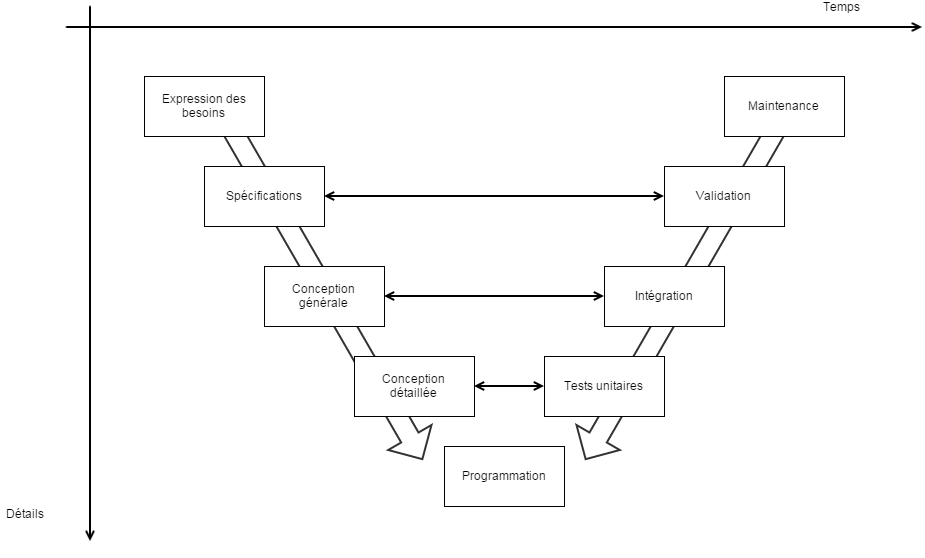
\includegraphics[width=14cm]{images/cycle_en_v.png}
  }
\end{figure}
\chapter{Plannification}
Ici un diagramme montrant mon planning durant le stage.
mars<->juin g1r6\\
juin->annomalie éligible g1r7\\
juillet<->aout g1r7
\chapter{Travail réalisé}
\section{Montée en compétence}
je vais parler de la prise en main des outils, des langages et la compréhension de geofibre.
\section{Développement}
Je parlerais des développements que j'ai fait pour al G1R6 (externalisation des paramètres du code en BDD).
Et des développement en G1R7 (Ajout du champ deployeur en BDD, sur l'IHM, script de recopie de données par ex)
\section{Intégration}
Je parlerais des tests d'integration, leurs niveau d'importance, le système de vagues, et un exemple de passage
\section{Corrections d'anomalies}
Je parlerais de comment on corrige une anomalie et un exemple.
